\section{Ejercicio 5}


Para este ejercicio se pedía ejecutar y graficar el lote de tareas del ejercicio 2 utilizando el scheduler \emph{Round-Robin} con quantum de 2, 5 y 10, y luego calcular la \textit{latencia}, el \textit{waiting time} y el tiempo total de ejecución de las tareas para cada quantum.

\subsection{Lote Ejecutado Con Quantum 2}

\begin{figure}[!h]
	\begin{center}
		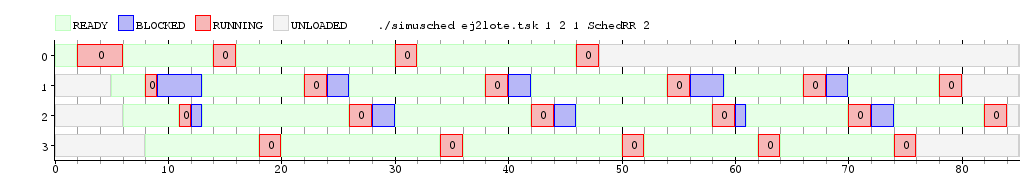
\includegraphics[width=500px]{imagenes/ej5_2.png}
		\caption{Ejecución del lote \emph{ej2lote} con quantum 2.}
		\label{fig:grafico_ej5_2}
	\end{center}
\end{figure}

%LATENCIA
\begin{center}
	\begin{tabular}{|c|c|c|c|c|}
		\hline
		\multicolumn{5}{|c|}{\textbf{Latencia}} \\
		\hline
		\textbf{Quantum} & \textbf{TaskCPU @0} & \textbf{TaskConsola @5} & \textbf{TaskConsola @6} & \textbf{TaskCPU @8} \\
		\hline
		2 & 2 & 3 & 5 & 10 \\
		\hline
	\end{tabular}
\end{center}

%WAITING TIME
\begin{center}
	\begin{tabular}{|c|c|c|c|c|}
		\hline
		\multicolumn{5}{|c|}{\textbf{Waiting Time}} \\
		\hline
		\textbf{Quantum} & \textbf{TaskCPU @0} & \textbf{TaskConsola @5} & \textbf{TaskConsola @6} & \textbf{TaskCPU @8} \\
		\hline
		2 & 38 & 51 & 59 & 58 \\
		\hline
	\end{tabular}
\end{center}

%TIEMPO TOTAL DE EJECUCION
\begin{center}
	\begin{tabular}{|c|c|c|c|c|}
		\hline
		\multicolumn{5}{|c|}{\textbf{Tiempo Total De Ejecución}} \\
		\hline
		\textbf{Quantum} & \textbf{TaskCPU @0} & \textbf{TaskConsola @5} & \textbf{TaskConsola @6} & \textbf{TaskCPU @8} \\
		\hline
		2 & 46 & 72 & 73 & 58 \\
		\hline
	\end{tabular}
\end{center}

\subsection{Lote Ejecutado Con Quantum 5}

\begin{figure}[!h]
	\begin{center}
		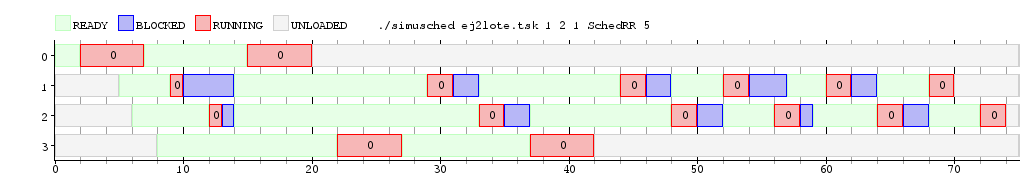
\includegraphics[width=500px]{imagenes/ej5_5.png}
		\caption{Ejecución del lote \emph{ej2lote} con quantum 5.}
		\label{fig:grafico_ej5_5}
	\end{center}
\end{figure}

%LATENCIA
\begin{center}
	\begin{tabular}{|c|c|c|c|c|}
		\hline
		\multicolumn{5}{|c|}{\textbf{Latencia}} \\
		\hline
		\textbf{Quantum} & \textbf{TaskCPU @0} & \textbf{TaskConsola @5} & \textbf{TaskConsola @6} & \textbf{TaskCPU @8} \\
		\hline
		5 & 2 & 4 & 6 & 14 \\
		\hline
	\end{tabular}
\end{center}

%WAITING TIME
\begin{center}
	\begin{tabular}{|c|c|c|c|c|}
		\hline
		\multicolumn{5}{|c|}{\textbf{Waiting Time}} \\
		\hline
		\textbf{Quantum} & \textbf{TaskCPU @0} & \textbf{TaskConsola @5} & \textbf{TaskConsola @6} & \textbf{TaskCPU @8} \\
		\hline
		5 & 10 & 39 & 49 & 22 \\
		\hline
	\end{tabular}
\end{center}

%TIEMPO TOTAL DE EJECUCION
\begin{center}
	\begin{tabular}{|c|c|c|c|c|}
		\hline
		\multicolumn{5}{|c|}{\textbf{Tiempo Total De Ejecución}} \\
		\hline
		\textbf{Quantum} & \textbf{TaskCPU @0} & \textbf{TaskConsola @5} & \textbf{TaskConsola @6} & \textbf{TaskCPU @8} \\
		\hline
		5 & 18 & 61 & 62 & 20 \\
		\hline
	\end{tabular}
\end{center}

\subsection{Lote Ejecutado Con Quantum 10}

\begin{figure}[!h]
	\begin{center}
		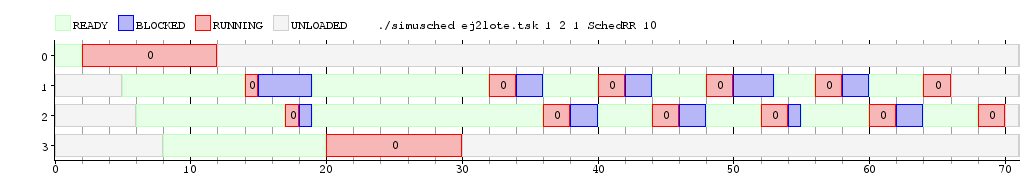
\includegraphics[width=500px]{imagenes/ej5_10.png}
		\caption{Ejecución del lote \emph{ej2lote} con quantum 10.}
		\label{fig:grafico_ej5_10}
	\end{center}
\end{figure}

%LATENCIA
\begin{center}
	\begin{tabular}{|c|c|c|c|c|}
		\hline
		\multicolumn{5}{|c|}{\textbf{Latencia}} \\
		\hline
		\textbf{Quantum} & \textbf{TaskCPU @0} & \textbf{TaskConsola @5} & \textbf{TaskConsola @6} & \textbf{TaskCPU @8} \\
		\hline
		10 & 2 & 9 & 11 & 12 \\
		\hline
	\end{tabular}
\end{center}

%WAITING TIME
\begin{center}
	\begin{tabular}{|c|c|c|c|c|}
		\hline
		\multicolumn{5}{|c|}{\textbf{Waiting Time}} \\
		\hline
		\textbf{Quantum} & \textbf{TaskCPU @0} & \textbf{TaskConsola @5} & \textbf{TaskConsola @6} & \textbf{TaskCPU @8} \\
		\hline
		10 & 2 & 37 & 45 & 12 \\
		\hline
	\end{tabular}
\end{center}

%TIEMPO TOTAL DE EJECUCION
\begin{center}
	\begin{tabular}{|c|c|c|c|c|}
		\hline
		\multicolumn{5}{|c|}{\textbf{Tiempo Total De Ejecución}} \\
		\hline
		\textbf{Quantum} & \textbf{TaskCPU @0} & \textbf{TaskConsola @5} & \textbf{TaskConsola @6} & \textbf{TaskCPU @8} \\
		\hline
		10 & 10 & 52 & 63 & 10 \\
		\hline
	\end{tabular}
\end{center}

